\section{Subgrupos, Generadores, Retículos y Grupos cíclicos}

\begin{ejercicio}\label{ej:3.1}
    Describir todos los elementos de los grupos alternados $A_n$, consistentes en las permutaciones pares del $S_n$ correspondiente, para:
    \begin{enumerate}
        \item $n = 2$.
        \begin{align*}
            S_2 &= \{1, (1\ 2)\}\\
            A_2 &= \{1\}
        \end{align*}
        \item $n = 3$.
        \begin{align*}
            S_3 &= \{1, (1\ 2), (1\ 3), (2\ 3), (1\ 2\ 3), (1\ 3\ 2)\}\\
            A_3 &= \{1, (1\ 2\ 3), (1\ 3\ 2)\}
        \end{align*}
        \item $n = 4$.
        \begin{align*}
            S_4 &= \{1, (1\ 2), (1\ 3), (1\ 4), (2\ 3), (2\ 4), (3\ 4), (1\ 2\ 3), (1\ 2\ 4), (1\ 3\ 2), (1\ 3\ 4),\\&\hspace{2cm} (1\ 4\ 2), (1\ 4\ 3), (2\ 3\ 4), (2\ 4\ 3), (1\ 2\ 3\ 4), (1\ 2\ 4\ 3), (1\ 3\ 2\ 4),\\&\hspace{2cm} (1\ 3\ 4\ 2), (1\ 4\ 2\ 3), (1\ 4\ 3\ 2), (1\ 2)(3\ 4), (1\ 3)(2\ 4), (1\ 4)(2\ 3)\}\\
            A_4 &= \{1, (1\ 2\ 3), (1\ 2\ 4), (1\ 3\ 2), (1\ 3\ 4), (1\ 4\ 2), (1\ 4\ 3), (2\ 3\ 4), (2\ 4\ 3),\\&\hspace{2cm} (1\ 2)(3\ 4), (1\ 3)(2\ 4), (1\ 4)(2\ 3)\}
        \end{align*}
    \end{enumerate}
\end{ejercicio}

\begin{ejercicio}\label{ej:3.2}
    Sea $D_n$ el grupo diédrico. Demostrar que el subgrupo de $D_n$ generado por los elementos $\{r^js, r^ks\}$ es todo el grupo $D_n$ siempre que $0 \leq j < k < n$ y $\mcd(k - j, n) = 1$.\\

    Haciendo uso de que $D_n = \langle r,s\rangle$, veamos que:
    \begin{align*}
        \langle r^js, r^ks\rangle &= D_n
    \end{align*}
    \begin{description}
        \item[$\subseteq)$] Como $r,s\in D_n$, entonces $r^js, r^ks\in D_n$. Por ser $D_n$ un grupo, en particular es cerrado para el producto y para inversos, por lo que $\langle r^js, r^ks\rangle\subseteq D_n$.
        
        \item[$\supseteq)$] Veamos en primer lugar que $r\in\langle r^js, r^ks\rangle$. Sabemos que:
        \begin{equation*}
            (r^js)^{-1} = sr^{-j}\in \langle r^js, r^ks\rangle
        \end{equation*}

        Por tanto, como $r^ks\in\langle r^js, r^ks\rangle$, entonces:
        \begin{equation*}
            r^ks(r^js)^{-1} = r^kssr^{-j} = r^{k-j}\in\langle r^js, r^ks\rangle
        \end{equation*}

        Como $\mcd(k-j,n)=1$, entonces existe $m\in\bb{Z}$, con $0\leq m<n$, tal que $m(k-j)=qn+1$ para algún $q\in\bb{Z}$. Por tanto:
        \begin{equation*}
            (r^{k-j})^m = r^{m(k-j)} = r^{qn+1} = r\in\langle r^js, r^ks\rangle
        \end{equation*}

        Por último, veamos que $s\in\langle r^js, r^ks\rangle$. Como $r\in\langle r^js, r^ks\rangle$, entonces:
        \begin{equation*}
            r^{n-j}r^js = r^{n-j+j}s = s\in\langle r^js, r^ks\rangle
        \end{equation*}

        Por tanto, $r,s\in\langle r^js, r^ks\rangle$, y por ser $D_n = \langle r,s\rangle$, entonces $D_n\subset \langle r^js, r^ks\rangle$.
    \end{description}
\end{ejercicio}

\begin{ejercicio}\label{ej:3.3}~
    \begin{enumerate}
        \item Demostrar que el subgrupo de $\SL_2(\bb{Z}_3)$ generado por los elementos
        \[
            i = \begin{pmatrix}
                0 & -1 \\
                1 & 0
            \end{pmatrix}, \quad j = \begin{pmatrix}
                1 & 1 \\
                1 & -1
            \end{pmatrix}
        \]
        es isomorfo al grupo cuaternio $Q_2$.\\

        Por la propiedad transitiva de la isomorfia, basta con encontrar un isomorfismo entre $\SL_2(\bb{Z}_3)$ y:
        \begin{equation*}
            Q_2^{abs} = \langle x,y\mid x^4=1,\ y^2=x^2,\ yx=x^{-1}y\rangle
        \end{equation*}

        Comprobamos que $i,j$ cumplen las relaciones de $Q_2^{abs}$:
        \begin{align*}
            i^2 &= \begin{pmatrix}
                -1 & 0 \\
                0 & -1
            \end{pmatrix}\\
            j^2 &= \begin{pmatrix}
                2 & 0 \\
                0 & 2
            \end{pmatrix} = \begin{pmatrix}
                -1 & 0 \\
                0 & -1
            \end{pmatrix}\\
            ji &= \begin{pmatrix}
                1 & -1 \\
                -1 & -1
            \end{pmatrix}\\
            i^3j &= \begin{pmatrix}
                1 & -1 \\
                -1 & -1
            \end{pmatrix}
        \end{align*}

        Por tanto, $i,j$ cumplen las relaciones de $Q_2^{abs}$. Por el Teorema de Teorema de Dyck, existe un único homomorfismo $f:Q_2^{abs}\to\langle i,j\rangle$ tal que $f(x)=i$ y $f(y)=j$.
        \begin{itemize}
            \item Como $i,j\in\langle i,j\rangle$ son un generador de $\langle i,j\rangle$, entonces se trata de un epimorfismo.
            \item Para terminar de ver que es un isomorfismo, basta con comprobar que $|Q_2^{abs}|=|\langle i,j\rangle|$. Sabemos que:
            \begin{align*}
                \langle i,j\rangle &= \{1,i,i^2,i^3,j,ij,i^2j,i^3j\}\\
                |Q_2^{abs}| &= 8 = |\langle i,j\rangle|
            \end{align*}

            Por tanto, $f$ es un isomorfismo.
        \end{itemize}
        Por tanto, $\langle i,j\rangle\cong Q_2^{abs}\cong Q_2$.
        \item Demostrar que $\SL_2(\bb{Z}_3)$ y $S_4$ son dos grupos de orden 24 que no son isomorfos.
        \begin{observacion}
            Demostrar que $S_4$ no puede contener a ningún subgrupo isomorfo a $Q_2$.
        \end{observacion}
        
        Tenemos que:
        \begin{equation*}
            Q_2 = \{\pm 1, \pm i, \pm j, \pm k\}
        \end{equation*}

        Los órdenes de los elementos de $Q_2$ son:
        \begin{equation*}
            O(\pm i)= O(\pm j)= O(\pm k)=4\qquad O(-1)=2
        \end{equation*}

        Supongamos ahora $\exists H\leq S_4$ tal que $H\cong Q_2$. Por lo pronto, sabemos que $1\in H$ y $|H|=8$.
        Además, como los isomorfismos mantienen los órdenes, sabemos que en $H$ habrá $6$ elementos distintos de orden 4 y $1$ de orden 2. Como en $S_4$ tan solo hay $6$ elementos de orden 4, entonces $H$ ha de contener a todos los elementos de orden 4 de $S_4$; es decir:
        \begin{equation*}
            \{1, (1\ 2\ 3\ 4), (1\ 2\ 4\ 3), (1\ 3\ 2\ 4), (1\ 3\ 4\ 2), (1\ 4\ 2\ 3), (1\ 4\ 3\ 2)\}\subseteq H
        \end{equation*}

        Por tanto, ya tenemos $7$ elementos de $H$, y sabemos que el restante es de orden $2$ (no sabemos si es una transposición o un producto de dos transposición disjuntas). Por ser $H$ un grupo, tenemos que es cerrado para productos, por lo que:
        \begin{equation*}
            (1\ 2\ 3\ 4)(1\ 2\ 4\ 3)=(1\ 3\ 2)\in H
        \end{equation*}
        No obstante, hemos encontrado un elemento de orden $3$ perteneciente a $H$, lo cual es una contradicción. Por tanto, no puede existir un subgrupo de $S_4$ isomorfo a $Q_2$.\\

        Para demostrar lo pedido, supongamos que $\exists f:\SL_2(\bb{Z}_3)\to S_4$ un isomorfismo, y consideramos la restricción a $Q=\langle i,j\rangle\cong Q_2$. Sabemos que la siguiente aplicación es un isomorfismo:
        \Func{f_{\big| Q}}{Q}{f_{\ast}(Q)}{x}{f(M)}

        Por tanto, $Q_2\cong Q\cong f_{\ast}(Q)$. Además, como $f_\ast$ es un homomorfismo y se tiene $Q< \SL_2(\bb{Z}_3)$, entonces $f_{\ast}(Q)< S_4$. Por tanto, hemos encontrado un subgrupo de $S_4$ isomorfo a $Q_2$, lo cual es una contradicción por lo que hemos demostrado anteriormente. Por tanto, $\SL_2(\bb{Z}_3)\ncong S_4$.
    \end{enumerate}
\end{ejercicio}

\begin{ejercicio}\label{ej:3.4}
    Razonar que un subconjunto no vacío $X \subseteq G$ de un grupo $G$ es un subgrupo de $G$ si, y sólo si, $X = \langle X \rangle$.
    \begin{description}
        \item[$\Longrightarrow)$] Supongamos que $X$ es un subgrupo de $G$, y veamos que $X = \langle X \rangle$. \begin{description}
            \item[$\subseteq)$] Por definición de subgrupo generado por un conjunto, $X\subseteq\langle X\rangle$.
            \item[$\supseteq)$] Veamos que $\langle X\rangle\subseteq X$. Dado $x\in \langle X\rangle$, entonces $x$ es una combinación de elementos de $X$ mediante el producto y el inverso. Por ser $X$ un subgrupo, en particular es un grupo, por lo que es cerrado para el producto y para inversos. Por tanto, $x\in X$.
        \end{description}

        Por tanto, $X = \langle X\rangle$.
        \item[$\Longleftarrow)$] Supongamos que $X = \langle X\rangle$, y veamos que $X$ es un subgrupo de $G$. Por definición, $\langle X\rangle$ es el menor subgrupo de $G$ que contiene a $X$. Por tanto, $X$ es un subgrupo de $G$.
    \end{description}
\end{ejercicio}

\begin{ejercicio}\label{ej:3.5}
    Sean $a, b \in G$ dos elementos de un grupo que conmutan entre sí, esto es, para los que $ab = ba$, y de manera que sus órdenes son primos relativos, esto es, $\mcd(O(a), O(b)) = 1$.
    \begin{enumerate}
        \item Razonar que $\langle a \rangle \cap \langle b \rangle = \{1\}$.
        
        Puesto que la intersección de dos subgrupos es un subgrupo, sabemos que $\langle a\rangle\cap\langle b\rangle$ es un subgrupo de $G$, y por tanto $1\in \langle a\rangle\cap\langle b\rangle\neq \emptyset$. Por tanto, podemos considerar $x\in \langle a\rangle\cap\langle b\rangle$.

        Como menciona el $\mcd(O(a),O(b))$, podemos considerar que ambos órdenes son finitos. Por el Teorema de Lagrange, sabemos que:
        \begin{align*}
            |\langle a\rangle\cap \langle b\rangle|&\mid |\langle a\rangle|=O(a)\\
            |\langle a\rangle\cap \langle b\rangle|&\mid |\langle b\rangle|=O(b)
        \end{align*}

        Por tanto, $|\langle a\rangle\cap \langle b\rangle|$ es divisor común de $O(a)$ y $O(b)$, y por ser $\mcd(O(a),O(b))=~1$, entonces $|\langle a\rangle\cap \langle b\rangle|=1$. Por tanto, $\langle a\rangle\cap \langle b\rangle=\{1\}$.

        \item Demostrar que $O(ab) = O(a)O(b)$.
        
        Puesto que conmutan, tenemos que:
        \begin{equation*}
            (ab)^k=a^kb^k\qquad \forall k\in\bb{Z}
        \end{equation*}

        Por comodidad, sean $O(a)=n$ y $O(b)=m$.
        \begin{equation*}
            (ab)^{nm}=a^{nm}b^{nm}=(a^n)^m(b^m)^n=1
        \end{equation*}

        Supongamos ahora $t\in \bb{N}$ tal que $(ab)^t=1$. 
        \begin{equation*}
            \hspace{-1cm}1=(ab)^t=a^tb^t\implies a^t=b^{-t}\in \langle a\rangle\cap \langle b\rangle=\{1\}\implies \left\{\begin{array}{c}
                a^t=1\Longrightarrow n\mid t\\
                a^t=1\Longrightarrow m\mid t
            \end{array}\right\}\stackrel{(\ast)}{\Longrightarrow} nm\mid t
        \end{equation*}
        donde en $(\ast)$ hemos usado que $\mcd(n,m)=1$. Por tanto:
        \begin{equation*}
            O(ab)=nm=O(a)O(b)
        \end{equation*}
    \end{enumerate}
\end{ejercicio}

\begin{ejercicio}\label{ej:3.6}
    Encontrar un grupo $G$ y elementos $a, b \in G$ tales que sus órdenes sean primos relativos, pero para los que no se verifique la igualdad $O(ab) = O(a)O(b)$ del ejercicio anterior.\\

    En primer lugar, hemos de tener que no conmuten. Por tanto, consideremos el grupo $S_3$ y los elementos:
    \begin{align*}
        a &= (1\ 2)\\
        b &= (1\ 2\ 3)
    \end{align*}

    Tenemos que $O(a)=2$ y $O(b)=3$, y por tanto $\mcd(O(a),O(b))=1$. Además, $O(a)O(b)=6$. Supongamos que $\exists \sigma\in S_3$ tal que $O(\sigma)=6$. Por tanto, el mínimo común múltiplo de los ciclos disjuntos que la descomponen debe ser 6. Sin embargo, esto no es posible, porque en $S_3$ tan solo hay elementos de orden 1, 2 y 3. Por tanto, $O(ab)\neq O(a)O(b)$.
\end{ejercicio}

\begin{ejercicio}\label{ej:3.7}
    Sea $G$ un grupo y $a, b \in G$ dos elementos de orden finito. ¿Es $ab$ necesariamente de orden finito?
    \begin{observacion}
        Considerar el grupo $\GL_2(\bb{Q})$ y los elementos
        \[
            a = \begin{pmatrix}
                0 & -1 \\
                1 & 0
            \end{pmatrix}, \quad b = \begin{pmatrix}
                0 & 1 \\
                -1 & 1
            \end{pmatrix}.
        \]
    \end{observacion}
    Calculemos el orden de $a$ y $b$:
    \begin{align*}
        a^2&=\begin{pmatrix}
            -1 & 0 \\
            0 & -1
        \end{pmatrix}=-I_2\implies O(a)=4\\
        b^2&=\begin{pmatrix}
            -1 & 1 \\
            -1 & 0
        \end{pmatrix}\\
        b^3&=\begin{pmatrix}
            -1 & 0 \\
            0 & -1
        \end{pmatrix}=-I_2\implies O(b)=6
    \end{align*}

    Calculamos ahora el orden de $ab$. Por inducción, demostraremos que:
    \begin{equation*}
        (ab)^n=\begin{pmatrix}
            1 & -n \\
            0 & 1
        \end{pmatrix}
    \end{equation*}
    \begin{itemize}
        \item \ul{Caso base:} $n=1$.
        \begin{equation*}
            (ab)^1=\begin{pmatrix}
                0 & -1 \\
                1 & 0
            \end{pmatrix}\begin{pmatrix}
                0 & 1 \\
                -1 & 1
            \end{pmatrix}=\begin{pmatrix}
                1 & -1 \\
                0 & 1
            \end{pmatrix}
        \end{equation*}

        \item \ul{Supuesto cierto para $n$, demostramos para $n+1$:}
        \begin{align*}
            (ab)^{n+1}&=(ab)^n(ab)=\begin{pmatrix}
                1 & -n \\
                0 & 1
            \end{pmatrix}\begin{pmatrix}
                1 & -1 \\
                0 & 1
            \end{pmatrix}
            =\begin{pmatrix}
                1 & -(n+1) \\
                0 & 1
            \end{pmatrix}
        \end{align*}
    \end{itemize}

    Por tanto, como en $(ab)^n\neq I_2$ para todo $n\in\bb{N}$, entonces $O(ab)=\infty$.
\end{ejercicio}

\begin{ejercicio}\label{ej:3.8}
    En el grupo $S_3$ se considera el conjunto
    \[
        H = \{1, (1\ 2\ 3), (1\ 3\ 2)\}.
    \]
    \begin{enumerate}
        \item Demostrar que $H$ es un subgrupo de $S_3$.
        
        Por ser $S_3$ finito, tan solo hemos de comprobar que $H$ es cerrado para el producto. Como vimos, no es necesario comprobar si uno de los elementos es el neutro.
        \begin{align*}
            (1\ 2\ 3)^2&=(1\ 3\ 2)\\
            (1\ 3\ 2)^2&=(1\ 2\ 3)\\
            (1\ 2\ 3)(1\ 3\ 2)&=1\\
            (1\ 3\ 2)(1\ 2\ 3)&=1
        \end{align*}

        Por tanto, $H< S_3$.
        \item Describir las diferentes clases de $S_3$ módulo $H$.
        
        Por el Teorema de Lagrange, sabemos que:
        \begin{equation*}
            |S_3|=[S_3:H]\cdot |H|\Longrightarrow [S_3:H]=\dfrac{6}{3}=2\Longrightarrow |S_3/\prescript{}{H}{\sim}| = |S_3/\sim_H|=2
        \end{equation*}

        Calculamos ahora las clases de equivalencia de $S_3/\prescript{}{H}{\sim}$:
        \begin{align*}
            1H &= \{1x\mid x\in H\} = \{1, (1\ 2\ 3), (1\ 3\ 2)\} = H\\
            (1\ 2)H &= \{(1\ 2)x\mid x\in H\} = \{(1\ 2), (1\ 2)(1\ 2\ 3), (1\ 2)(1\ 3\ 2)\} = \{(1\ 2), (2\ 3), (1\ 3)\}\neq H
        \end{align*}
        Como ya hemos encontrado dos clases de equivalencia distintas, entonces hemos encontrado todas las posibles.
        \begin{equation*}
            S_3/\prescript{}{H}{\sim} = \{H, (1\ 2)H\}
        \end{equation*}

        Calculamos ahora las clases de equivalencia de $S_3/\sim_H$:
        \begin{align*}
            H1 &= \{x1\mid x\in H\} = \{1, (1\ 2\ 3), (1\ 3\ 2)\} = H\\
            H(1\ 2) &= \{x(1\ 2)\mid x\in H\} = \{(1\ 2), (1\ 2\ 3)(1\ 2), (1\ 3\ 2)(1\ 2)\} = \{(1\ 2), (1\ 3), (2\ 3)\}\neq H
        \end{align*}

        Por tanto, hemos encontrado todas las clases de equivalencia de $S_3/\sim_H$.
        \begin{equation*}
            S_3/\sim_H = \{H, H(1\ 2)\}
        \end{equation*}
    \end{enumerate}
\end{ejercicio}

\begin{ejercicio}\label{ej:3.9}
    Sea $G$ un grupo finito.
    \begin{enumerate}
        \item Demostrar que si $H \leq G$ es un subgrupo, entonces $[G : H] = |G|$ si, y sólo si, $H = \{1\}$, mientras que $[G : H] = 1$ si, y sólo si, $H = G$.\\
        
        Demostremos en primer lugar que $[G:H]=|G|\iff H=\{1\}$. Por el Teorma de Lagrange, sabemos que $|G|=[G:H]\cdot |H|$. Por tanto:
        \begin{equation*}
            [G:H]=\dfrac{|G|}{|H|}=|G|\iff |G|=|G|\ |H|\iff |H|=1\iff H=\{1\}
        \end{equation*}
        donde, desde el inicio, hemos usado que $|G|, |H|\neq 0$.\\

        De nuevo, por el Teorema de Lagrange, sabemos que $|G|=[G:H]\cdot |H|$. Por tanto:
        \begin{equation*}
            [G:H]=\dfrac{|G|}{|H|}=1\iff |G|=|H|
        \end{equation*}
        Como además $H\subset G$ por ser subgrupo, tenemos que $[G:H]=1$ si y solo si $H=G$.
        \item Demostrar que si se tienen subgrupos $G_2 \leq G_1 \leq G$, entonces
        \[
            [G : G_2] = [G : G_1][G_1 : G_2],
        \]
        
        Por un lado, como $G_2\leq G$, entonces:
        \begin{equation*}
            |G|=[G:G_2]\cdot |G_2|
        \end{equation*}

        Por otro lado, como $G_1\leq G$, y $G_2\leq G_1$, entonces:
        \begin{equation*}
            |G|=[G:G_1]\cdot |G_1|=[G:G_1][G_1:G_2]\cdot |G_2|
        \end{equation*}

        Uniendo ambos resultados, tenemos que:
        \begin{equation*}
            [G:G_2]=[G:G_1][G_1:G_2]
        \end{equation*}
        \item Demostrar que si se tiene una cadena descendente de subgrupos de la forma
        \[
            G = G_0 \geq G_1 \geq \cdots \geq G_{r - 1} \geq G_r,
        \]
        entonces
        \[
            [G : G_r] = \prod_{i = 0}^{r - 1}[G_i : G_{i + 1}].
        \]

        Demotrsamos por inducción sobre $r$:
        \begin{itemize}
            \item \ul{$r=2$:} $G=G_0\geq G_1\geq G_2$. Por el apartado anterior, sabemos que:
            \begin{equation*}
                [G:G_2]=[G:G_1][G_1:G_2]
            \end{equation*}

            \item \ul{Supuesto cierto para $r$, demostramos para $r+1$:}
            Por hipótesis de inducción, sabemos que:
            \begin{equation*}
                [G:G_r]=\prod_{i=0}^{r-1}[G_i:G_{i+1}]
            \end{equation*}

            Por otro lado, como $G_{r+1}\leq G_r\leq G$, aplicando el apartado anterior, tenemos que:
            \begin{equation*}
                [G:G_{r+1}]=[G:G_r][G_r:G_{r+1}]
            \end{equation*}

            Uniendo ambos resultados, tenemos que:
            \begin{equation*}
                [G:G_{r+1}]=\prod_{i=0}^{r-1}[G_i:G_{i+1}]\cdot [G_r:G_{r+1}]
                = \prod_{i=0}^{r}[G_i:G_{i+1}]
            \end{equation*}
        \end{itemize}
        \item Demostrar que si se tiene una cadena descendente de subgrupos de la forma
        \[
            G = G_0 \geq G_1 \geq \cdots \geq G_{r - 1} \geq G_r = \{1\},
        \]
        entonces
        \[
            |G| = \prod_{i = 0}^{r - 1}[G_i : G_{i + 1}].
        \]

        Por el primer apartado, como $G_r=\{1\}$, entonces $[G:G_r]=|G|$. Por tanto, aplicando el apartado anterior, tenemos que:
        \begin{equation*}
            |G|=\prod_{i=0}^{r-1}[G_i:G_{i+1}]
        \end{equation*}
    \end{enumerate}
\end{ejercicio}

\begin{ejercicio}\label{ej:3.10}~
    \begin{enumerate}
        \item Demostrar que si $G$ es un grupo de orden 4, entonces se tiene que o bien $G$ es cíclico, o bien es isomorfo al grupo de Klein.
        
        Como $|G|=4$, entonces $O(x)\mid 4$ para todo $x\in G$. Por tanto, $O(x)\in \{1,2,4\}$. Consideramos los siguientes casos:
        \begin{itemize}
            \item \ul{Supongamos $\exists x\in G\mid O(x)=4$:}
            
            En este caso, como $x$ tiene 4 potencias distintas, entonces:
            \begin{equation*}
                \langle x\rangle = \{1,x,x^2,x^3\}\subset G
            \end{equation*}

            Como además $|\langle x\rangle|=4=|G|$, entonces $G=\langle x\rangle$. Por tanto, $G$ es cíclico, $G=C_4$.

            \item \ul{Supongamos $\nexists x\in G\mid O(x)=4$:}
            
            En este caso, $\forall x\in G$, $O(x)\in\{1,2\}$. Como $O(x)=1\iff x=1$, entonces $G$ tiene $3$ elementos de orden 2. Sea $x\in G$ tal que $O(x)=2$.
            
            En este caso, $\langle x\rangle = \{1,x\}\subset G$. Como $|G|=4$, ha de existir un elemento $y\in G$ tal que $y\notin\langle x\rangle$ y $O(y)=2$.

            Veamos que $G$ cumple las relaciones del grupo de Klein abstracto:
            \begin{align*}
                V^{\text{abs}} = \langle a,b\mid a^2=b^2=1,\ ab=ba\rangle
            \end{align*}

            Sabemos que $x^2=y^2=1$. Ahora, nos falta ver que $xy=yx$. Como $xy\in G$, entonces $O(xy)\in\{1,2\}$. En cualquier caso, $(xy)^2=1$, por lo que:
            \begin{equation*}
                xyxy=1\Longrightarrow yxy=x\Longrightarrow xy=yx
            \end{equation*}

            Por tanto, por el Teorema de Dyck, $G\cong V^{\text{abs}}\cong V$.
        \end{itemize}
        \item Demostrar que si $G$ es un grupo de orden 6, entonces se tiene que o bien $G$ es cíclico, o bien es isomorfo al grupo diédrico $D_3$.
        
        Seguiremos la misma estrategia que en el apartado anterior. Como $|G|=6$, entonces $O(x)\mid 6$ para todo $x\in G$. Por tanto, $O(x)\in \{1,2,3,6\}$. Consideramos los siguientes casos:
        \begin{itemize}
            \item \ul{Supongamos $\exists x\in G\mid O(x)=6$:}
            
            En este caso, como $x$ tiene 6 potencias distintas, entonces:
            \begin{equation*}
                \langle x\rangle = \{1,x,x^2,x^3,x^4,x^5\}\subset G
            \end{equation*}

            Como además $|\langle x\rangle|=6=|G|$, entonces $G=\langle x\rangle$. Por tanto, $G$ es cíclico, $G=C_6$.

            \item \ul{Supongamos $\nexists x\in G\mid O(x)=6$:}
            
            En este caso, $\forall x\in G$, $O(x)\in\{1,2,3\}$. Como $O(x)=1\iff x=1$, entonces $G$ tiene $5$ elementos cuyo orden es $2$ o $3$.
            \begin{itemize}
                \item \ul{Supongamos $\nexists x\in G\mid O(x)=3$:}
                
                Entonces, $G$ tiene $5$ elementos de orden 2. Sea $x\in G$ tal que $O(x)=2$.
                \begin{equation*}
                    \langle x\rangle = \{1,x\}\subset G
                \end{equation*}

                Como $|G|=6$, ha de existir un elemento $y\in G$ tal que $y\notin\langle x\rangle$ y $O(y)=2$. Veamos que $xy\notin \{1,x,y\}$.
                \begin{itemize}
                    \item Si $xy=1$, entonces $y=x^{-1}=x$, lo cual es una contradicción.
                    \item Si $xy=x$, entonces $y=1$, lo cual es una contradicción.
                    \item Si $xy=y$, entonces $x=1$, lo cual es una contradicción.
                \end{itemize}
                Por tanto, tenemos que:
                \begin{equation*}
                    \langle x,y\rangle = \{1,x,y,xy\}\subset G
                \end{equation*}

                Por tanto, hemos encontrado un subgrupo de $G$ de orden 4, pero esto es una contradicción, porque por el Teorema de Lagrange, el orden de un subgrupo ha de dividir al orden del grupo.

                \item \ul{Supongamos $\nexists x\in G\mid O(x)=2$:}
                
                En este caso, $G$ tiene $5$ elementos de orden 3. Sea $x\in G$ tal que $O(x)=3$.
                \begin{equation*}
                    \langle x\rangle = \{1,x,x^2\}\subset G
                \end{equation*}

                Como $|G|=6$, ha de existir un elemento $y\in G$ tal que $y\notin\langle x\rangle$ y $O(y)=3$. Veamos que $xy\notin \{1,x,x^2, y, y^2\}$.
                \begin{itemize}
                    \item Si $xy=1$, entonces $y=x^{-1}=x^2$, lo cual es una contradicción.
                    \item Si $xy=x$, entonces $y=1$, lo cual es una contradicción.
                    \item Si $xy=x^2$, entonces $y=x$, lo cual es una contradicción.
                    \item Si $xy=y$, entonces $x=1$, lo cual es una contradicción.
                    \item Si $xy=y^2$, entonces $x=y$, lo cual es una contradicción.
                \end{itemize}

                Por tanto, tenemos que $\{1,x,x^2,y,y^2,xy\}\subset G$. Como $|G|=6$, entonces $G=\{1,x,x^2,y,y^2,xy\}$. Veamos que $x^2y\notin G$:
                \begin{itemize}
                    \item Si $x^2y=1$, entonces $y=x$, lo cual es una contradicción.
                    \item Si $x^2y=x$, entonces $y=x^2$, lo cual es una contradicción.
                    \item Si $x^2y=x^2$, entonces $y=1$, lo cual es una contradicción.
                    \item Si $x^2y=y$, entonces $x^2=1$, lo cual es una contradicción.
                    \item Si $x^2y=y^2$, entonces $x^2=y$, lo cual es una contradicción.
                    \item Si $x^2y=xy$, entonces $x=1$, lo cual es una contradicción.
                \end{itemize}
                Por tanto, $G$ no es cerrado para el producto, lo cual es una contradicción.

                \item Por tanto, $\exists x\in G\mid O(x)=3$ y $\exists y\in G\mid O(y)=2$. Comprobemos que $G$ cumple las relaciones del grupo diédrico $D_3$:
                \begin{equation*}
                    D_3 = \langle r,s\mid r^3=s^2=1,\ sr=r^2s\rangle
                \end{equation*}

                Veamos en primer lugar los elementos de $G$. Sabemos que $\{1,x,x^2\}\subset~G$. Veamos ahora que $y$ no puede ser uno de estos elementos:
                \begin{equation*}
                    y=x^2\Longrightarrow 1=y^2=x^4=x\Longrightarrow x=1
                \end{equation*}
                Por tanto, $y\notin \{1,x,x^2\}$, y tenemos $\{1,x,x^2,y\}\subset G$. Veamos ahora que $xy\notin \{1,x,x^2,y\}$:
                \begin{itemize}
                    \item Si $xy=1$, entonces $y=x$, lo cual es una contradicción.
                    \item Si $xy=x$, entonces $y=1$, lo cual es una contradicción.
                    \item Si $xy=x^2$, entonces $y=x$, lo cual es una contradicción.
                    \item Si $xy=y$, entonces $x=1$, lo cual es una contradicción.
                \end{itemize}

                Por tanto, $\{1,x,x^2,y,xy\}\subset G$. Veamos ahora que $x^2y\notin \{1,x,x^2,y,xy\}$:
                \begin{itemize}
                    \item Si $x^2y=1$, entonces $y=x$, lo cual es una contradicción.
                    \item Si $x^2y=x$, entonces $y=x^2$, lo cual es una contradicción.
                    \item Si $x^2y=x^2$, entonces $y=1$, lo cual es una contradicción.
                    \item Si $x^2y=y$, entonces $x^2=1$, lo cual es una contradicción.
                    \item Si $x^2y=xy$, entonces $x=1$, lo cual es una contradicción.
                \end{itemize}

                Por tanto, $\{1,x,x^2,y,xy,x^2y\}\subset G$. Como $|G|=6$, entonces:
                \begin{equation*}
                    G=\{1,x,x^2,y,xy,x^2y\}
                \end{equation*}

                Como $G$ es un grupo, $yx\in G$. Veamos el valor de $yx$:
                \begin{itemize}
                    \item Si $yx=1$, entonces $y=x$, lo cual es una contradicción.
                    \item Si $yx=x$, entonces $y=1$, lo cual es una contradicción.
                    \item Si $yx=x^2$, entonces $y=x$, lo cual es una contradicción.
                    \item Si $yx=y$, entonces $x=1$, lo cual es una contradicción.
                    \item Si $yx=xy$, entonces $G$ es abeliano. En este caso, veamos que $O(xy)=6$:
                    \begin{equation*}
                        (xy)^2=x^2\qquad 
                        (xy)^3=y\qquad 
                        (xy)^4=x\qquad 
                        (xy)^5=x^2y\qquad 
                        (xy)^6=1
                    \end{equation*}
                    Por tanto, $O(xy)=6$, pero habíamos supuesto que $\nexists x\in G$ tal que $O(x)=6$. Por tanto, hemos llegado a una contradicción.
                \end{itemize}

                Por tanto, como $yx\in G$, tan solo queda la opción de que $yx=x^2y$. Por tanto, $G$ cumple las relaciones del grupo diédrico $D_3$. Como además $\langle x,y\rangle$ es un grupo de generadores de $G$ y $|G|=|D_3|=6$, por el Teorema de Dyck, $G\cong D_3$.
            \end{itemize}

        \end{itemize}
    \end{enumerate}
\end{ejercicio}

\begin{ejercicio}\label{ej:3.11}
    Describir los retículos de subgrupos de los siguientes grupos:
    \begin{enumerate}
        \item El grupo $V$ de Klein.
        \item El grupo simétrico $S_3$.
        \item El grupo diédrico $D_4$.
        \item El grupo cuaternio $Q_2$.
        \item El grupo alternado $A_4$.
    \end{enumerate}

    % // TODO: Hacer
\end{ejercicio}

\begin{ejercicio}\label{ej:3.12}
    Fijado un número primo $p$, describe el retículo de subgrupos del grupo cíclico $C_{p^n}$. En particular, describe el retículo de subgrupos del grupo cíclico $C_8$.\\

    Sabemos que, para cada divisor de $p^n$, existe un subgrupo de $C_{p^n}$ de ese orden. En concreto, los únicos subgrupos de $C_{p^n}$ son los de la forma $\langle x^{p^k}\rangle$ con $k\in \{0,\ldots,n\}$. Además:
    \begin{equation*}
        O(x^{p^k})=\dfrac{O(x)}{\mcd(O(x),p^k)}=\dfrac{p^n}{\mcd(p^n,p^k)}=\dfrac{p^n}{p^k}=p^{n-k}
    \end{equation*}

    Por tanto, $\langle x^{p^k}\rangle=C_{p^{n-k}}$. Además, fijado $k\in \{0,\ldots,n\}$, tenemos que $\langle x^{p^{k+1}}\rangle\subset \langle x^{p^{k}}\rangle$, puesto que $x^{p^{k+1}}=(x^{p^k})^{p}$.    
    Por tanto, el retículo de subgrupos de $C_{p^n}$ es el de la Figura~\ref{fig:ej12}.
    \begin{figure}
        \centering
        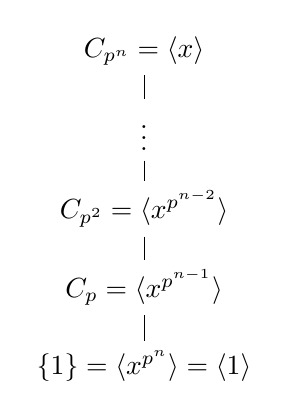
\begin{tikzpicture}[node distance=1cm]
            \node (G)  {$C_{p^n}=\langle x\rangle$};
            \node[below of=G] (p) {$\vdots$};
            \node[below of=p] (p2) {$C_{p^2}= \langle x^{p^{n-2}}\rangle$};
            \node[below of=p2] (p1) {$C_{p}= \langle x^{p^{n-1}}\rangle$};
            \node[below of=p1] (1) {$\{1\}= \langle x^{p^{n}}\rangle= \langle 1\rangle$};

            \draw (G) -- (p);
            \draw (p) -- (p2);
            \draw (p2) -- (p1);
            \draw (p1) -- (1);
        \end{tikzpicture}
        \caption{Retículo de subgrupos de $C_{p^n}$ para el Ejercicio~\ref{ej:3.12}.}
        \label{fig:ej12}
    \end{figure}

    En particular, para $C_8$, tenemos que $p=2$ y $n=3$. Por tanto, el retículo de subgrupos de $C_8$ es el de la Figura~\ref{fig:ej12_8}.
    \begin{figure}
        \centering
        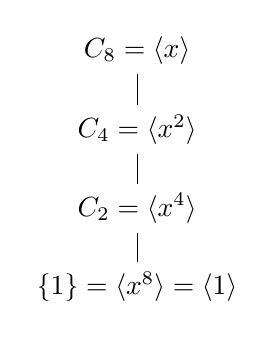
\begin{tikzpicture}[node distance=1cm]
            \node (G)  {$C_8=\langle x\rangle$};
            \node[below of=G] (p2) {$C_{4}= \langle x^{2}\rangle$};
            \node[below of=p2] (p1) {$C_{2}= \langle x^{4}\rangle$};
            \node[below of=p1] (1) {$\{1\}= \langle x^{8}\rangle= \langle 1\rangle$};

            \draw (G) -- (p2);
            \draw (p2) -- (p1);
            \draw (p1) -- (1);
        \end{tikzpicture}
        \caption{Retículo de subgrupos de $C_8$ para el Ejercicio~\ref{ej:3.12}.}
        \label{fig:ej12_8}
    \end{figure}
\end{ejercicio}

\begin{ejercicio}\label{ej:3.13}
    Demostrar que un grupo finito $G \neq \{1\}$ carece de subgrupos propios, esto es, que su retículo de subgrupos es el de la Figura~\ref{fig:ej13} si, y sólo si, $G = C_p$ es un grupo cíclico de orden primo.
    \begin{figure}
        \centering
        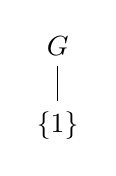
\begin{tikzpicture}[node distance=1cm]
            \node (G)  {$G$};
            \node[below of=G] (1) {$\{1\}$};

            \draw (G) -- (1);
        \end{tikzpicture}
        \caption{Retículo de subgrupos de para el Ejercicio~\ref{ej:3.13}.}
        \label{fig:ej13}
    \end{figure}

    \begin{description}
        \item[$\Longrightarrow)$] Supongamos que $G$ es un grupo finito que carece de subgrupos propios. Como $G\neq \{1\}$, sea $x\in G\setminus \{1\}$. Entonces, $\langle x\rangle\neq \{1\}$ es un subgrupo de $G$; y como este no es propio, entonces $\langle x\rangle=G$. Por tanto, $G$ es cíclico.
        
        Por último, por ser $G$ cíclico sabemos que, por cada divisor de $|G|$, existe un subgrupo de $G$ de ese orden. Como $G$ no tiene subgrupos propios, entonces los únicos divisores de $|G|$ son $1$ y $|G|$. Por tanto, $|G|$ es primo.

        \item[$\Longleftarrow)$] Supongamos que $G=C_p$ es un grupo cíclico de orden primo. Sabemos que, por cada divisor de $|G|$, existe un subgrupo de $G$ de ese orden. Como $|G|=p$ es primo, entonces los únicos divisores de $|G|$ son $1$ y $|G|$. Por tanto, $G$ carece de subgrupos propios.
    \end{description}
\end{ejercicio}

\begin{ejercicio}\label{ej:3.14}
    Describir los retículos de subgrupos de los grupos cíclicos siguentes:
    \begin{enumerate}
        \item $C_6$.
        
        Sabemos que los subgrupos propios de $C_6$ son de la forma $\langle x^k\rangle$ con $k\in \{2,3\}$. Además, $O(x^k)=\frac{6}{\mcd(6,k)}=\frac{6}{k}$. Por tanto, estos son:
        \begin{align*}
            \langle x^2\rangle &= \{1,x^2,x^4\}\\
            \langle x^3\rangle &= \{1,x^3\}
        \end{align*}

        Por tanto, el retículo de subgrupos de $C_6$ es el de la Figura~\ref{fig:ej14_6}.
        \begin{figure}
            \centering
            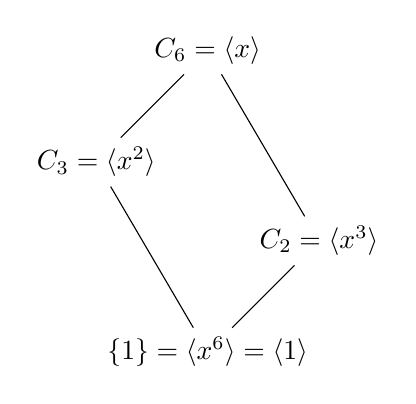
\begin{tikzpicture}[node distance=2cm]
                \node (G)  {$C_6=\langle x\rangle$};
                \node[below left of=G] (p2) {$C_{3}= \langle x^{2}\rangle$};
                \node[below right of=G, yshift=-1cm] (p1) {$C_{2}= \langle x^{3}\rangle$};
                \node[below left of=p1] (1) {$\{1\}= \langle x^{6}\rangle= \langle 1\rangle$};
    
                \draw (G) -- (p2);
                \draw (G) -- (p1);
                \draw (p2) -- (1);
                \draw (p1) -- (1);
            \end{tikzpicture}
            \caption{Retículo de subgrupos de $C_6$ para el Ejercicio~\ref{ej:3.14}.}
            \label{fig:ej14_6}
        \end{figure}
        \item $C_{12}$.
        
        Sabemos que los subgrupos propios de $C_{12}$ son de la forma $\langle x^k\rangle$ con $k\in \{2,3,4,6\}$. Además, $O(x^k)=\frac{12}{\mcd(12,k)}=\frac{12}{k}$. Por tanto, estos son:
        \begin{align*}
            \langle x^2\rangle &= \{1,x^2,x^4,x^6,x^8,x^{10}\}\\
            \langle x^3\rangle &= \{1,x^3,x^6,x^9\}\\
            \langle x^4\rangle &= \{1,x^4,x^8\}\\
            \langle x^6\rangle &= \{1,x^6\}
        \end{align*}

        Por tanto, el retículo de subgrupos de $C_{12}$ es el de la Figura~\ref{fig:ej14_12}.
        \begin{figure}
            \centering
            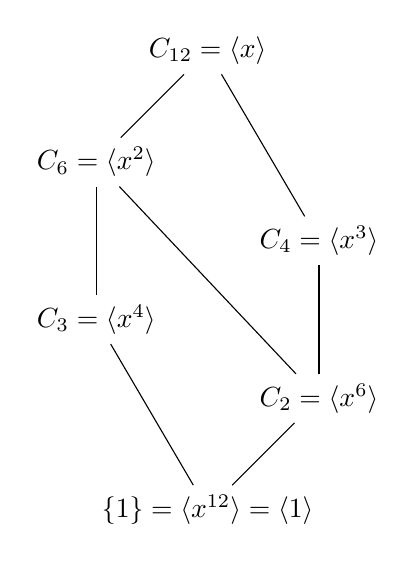
\begin{tikzpicture}[node distance=2cm]
                \node (G)  {$C_{12}=\langle x\rangle$};
                \node[below left of=G] (p2) {$C_{6}= \langle x^{2}\rangle$};
                \node[below right of=G, yshift=-1cm] (p1) {$C_{4}= \langle x^{3}\rangle$};
                \node[below of=p2] (p3) {$C_{3}= \langle x^{4}\rangle$};
                \node[below of=p1] (p4) {$C_{2}= \langle x^{6}\rangle$};
                \node[below left of=p4] (1) {$\{1\}= \langle x^{12}\rangle= \langle 1\rangle$};
    
                \draw (G) -- (p2);
                \draw (G) -- (p1);
                \draw (p2) -- (p3);
                \draw (p1) -- (p4);
                \draw (p4) -- (p2);
                \draw (p3) -- (1);
                \draw (p4) -- (1);
            \end{tikzpicture}
            \caption{Retículo de subgrupos de $C_{12}$ para el Ejercicio~\ref{ej:3.14}.}
            \label{fig:ej14_12}
        \end{figure}
    \end{enumerate}
\end{ejercicio}

\begin{ejercicio}\label{ej:3.15}
    Se considera el grupo cíclico $C_{136}$ de orden 136, con generador $t$. ¿Qué relación hay entre los subgrupos $H_1 = \langle t^{48}, t^{72} \rangle$ y $H_2 = \langle t^{46} \rangle$?\\

    Estudiamos en primer lugar el grupo $H_2$. Como $O(t)=136$, entonces:
    \begin{equation*}
        H_2 = \langle t^{46}\rangle = \langle t^{\mcd(136,46)}\rangle = \langle t^2\rangle
    \end{equation*}

    Por otro lado:
    \begin{align*}
        H_1 &= \langle t^{48}, t^{72}\rangle = \langle t^{48}\rangle \vee \langle t^{72}\rangle = \langle t^{\mcd(136,48)}\rangle \vee \langle t^{\mcd(136,72)}\rangle\\
        &= \langle t^8\rangle \vee \langle t^{8}\rangle = \langle t^8\rangle
    \end{align*}

    Por tanto, se nos pide estudiar la relación entre los subgrupos $\langle t^2\rangle$ y $\langle t^8\rangle$. Puesto que $t_8\in \langle t^2\rangle$, entonces:
    \begin{equation*}
        H_1 = \langle t^8\rangle < \langle t^2\rangle = H_2
    \end{equation*}
\end{ejercicio}

\begin{ejercicio}\label{ej:3.16}
    Demostrar que el grupo de unidades $\bb{Z}_7^\times$ es un grupo cíclico.\\

    Veamos que $O(5)=6$:
    \begin{align*}
        5^2 &= 4\\
        5^3 &= 6\\
        5^4 &= 2\\
        5^5 &= 3\\
        5^6 &= 1
    \end{align*}

    Por tanto, $\bb{Z}_7^\times = \langle 5\rangle$ es un grupo cíclico.
\end{ejercicio}

\begin{ejercicio}\label{ej:3.17}
    Sea $G$ un grupo y sea $C_n$ el grupo cíclico de orden $n$ generado por $x$. Demostrar que:
    \begin{enumerate}
        \item Si $\theta : C_n \to G$ es un homomorfismo de grupos, entonces:
        \begin{equation*}
            O(\theta(x))\mid n, \quad \text{y} \quad \theta(x^k) = \theta(x)^k \quad \forall k \in \{0, \ldots, n - 1\}.
        \end{equation*}

        Para la primera parte, queremos ver que $(\theta(x))^n=1$. Sabemos que:
        \begin{equation*}
            1 = \theta(1) = \theta(x^n) = \theta(x)^n\Longrightarrow
            O(\theta(x))\mid n
        \end{equation*}

        Para ver el segundo resultado, es suficiente ver que, por ser un homomorfismo, de hecho se tiene para todo $k\in \bb{Z}$. 

        \item Para cada $g \in G$ tal que $O(g) \mid n$, existe un único homomorfismo de grupos $\theta_g : C_n \to G$ tal que $\theta_g(x) = g$.
        
        Veamos que $g^n=1$. Como $O(g)\mid n$, existe $m\in \bb{Z}$ tal que $n=m\cdot O(g)$. Por tanto:
        \begin{equation*}
            g^n = g^{m\cdot O(g)} = (g^{O(g)})^m = 1^m = 1
        \end{equation*}

        Por tanto, por el Teorema de Dyck, existe un único homomorfismo de grupos $\theta_g : C_n \to G$ tal que $\theta_g(x) = g$.
        
        \item Si $g \in G$ es tal que $O(g) \mid n$, entonces el morfismo $\theta_g$ es monomorfismo si, y sólo si, $O(g) = n$.
        \begin{description}
            \item[$\Longrightarrow)$] Supongamos que $\theta_g$ es monomorfismo, y veamos que $O(g)=n$. Como $O(g)\mid n$, entonces $O(g)\leq n$. Supongamos ahora $m\in \bb{Z}$ tal que $g^m=1$. Entonces:
            \begin{equation*}
                \theta_g(1)=1 =g^m=\theta_g(x)^m=\theta_g(x^m)
            \end{equation*}

            Por ser $\theta_g$ monomorfismo, entonces $x^m=1$, y por tanto $m\geq n$. Por tanto, $O(g)=n$.


            \item[$\Longleftarrow)$] Supongamos que $O(g)=n$, y veamos que $\theta_g$ es monomorfismo. Para ello, calculemos el núcleo de $\theta_g$:
            \begin{align*}
                \ker(\theta_g) &= \{x\in C_n\mid \theta_g(x)=1\}
                = \{x^k\mid k\in \{0,\ldots,n-1\},\quad \theta_g(x^k)=1\}\\
                &= \{x^k\mid k\in \{0,\ldots,n-1\},\quad g^k=1\}
            \end{align*}
            Como $O(g)=n$, entonces $g^k=1\iff k=0$. Por tanto, $\ker(\theta_g)=\{1\}$, y por tanto $\theta_g$ es monomorfismo.
        \end{description}
        
        \item Existe un isomorfismo de grupos
        \begin{equation*}
            \cc{U}(\bb{Z}_n) \cong \Aut(C_n),
        \end{equation*}
        dado por $r \mapsto f_r$ para cada $r = 1, \ldots, n-1$ con $\mcd(r, n) = 1$, donde el automorfismo $f_r$ se define mediante $f_r(x) = x^r$.

        En particular, $\Aut(C_n)$ es un grupo abeliano de orden $\varphi(n)$.


        % // TODO: Por aquí
    \end{enumerate}
\end{ejercicio}

\begin{ejercicio}\label{ej:3.18}~
    \begin{enumerate}
        \item Describir explícitamente el grupo de automorfismos $\Aut(C_8)$.
        
        \item Demostrar que $\Aut(C_8)$ es isomorfo al grupo de Klein.
    \end{enumerate}
\end{ejercicio}